\documentclass[10pt,aspectratio=169]{beamer}
%\documentclass[12pt,aspectratio=169]{beamer}

%\mode<presentation>

\usepackage{graphicx}
\usepackage{breqn}
\usepackage{bm}
\usepackage{color}
\usepackage{tabularx}

\usepackage{listings}
\lstset{language=C++}

\usepackage{mathtools}
\DeclarePairedDelimiter\ceil{\lceil}{\rceil}
\DeclarePairedDelimiter\floor{\lfloor}{\rfloor}


\usepackage{listings}

%\usepackage[utf8]{inputenc}
\definecolor{bluekeywords}{rgb}{0.63, 0.79, 0.95}
\definecolor{greencomments}{rgb}{0,0.5,0}
\definecolor{redstrings}{rgb}{0.64,0.08,0.08}
\definecolor{xmlcomments}{rgb}{0.5,0.5,0.5}
\definecolor{types}{rgb}{0.17,0.57,0.68}
\lstset{language=C++,
captionpos=b,
%numbers=left,
%numberstyle=\tiny,
frame=single,
showspaces=false,
showtabs=false,
breaklines=true,
showstringspaces=false,
breakatwhitespace=true,
escapeinside={(*@}{@*)},
commentstyle=\color{greencomments},
morekeywords={partial, var, value, get, set},
keywordstyle=\color{bluekeywords},
stringstyle=\color{redstrings},
basicstyle=\ttfamily\small,
}

\usepackage[yyyymmdd]{datetime}
\renewcommand{\dateseparator}{--}

%\usepackage[inline]{asymptote}
\usepackage{asymptote}
\def\asylatexdir{}
\def\asydir{}

\renewcommand{\thefootnote}{\fnsymbol{footnote}}

\def\clap#1{\hbox to 0pt{\hss#1\hss}}
\def\mathllap{\mathpalette\mathllapinternal}
\def\mathrlap{\mathpalette\mathrlapinternal}
\def\mathclap{\mathpalette\mathclapinternal}
\def\mathllapinternal#1#2{\llap{$\mathsurround=0pt#1{#2}$}}
\def\mathrlapinternal#1#2{\rlap{$\mathsurround=0pt#1{#2}$}}
\def\mathclapinternal#1#2{\clap{$\mathsurround=0pt#1{#2}$}}

\def\p{\pause}

\def\({\left(}
\def\){\right)}
\def\[{\left[}
\def\]{\right]}

\def\no#1{\nobreak{#1}} % stop equation breaking in dmath

\begin{asydef}
  // Global Asymptote definitions can be put here.
  import three;
  usepackage("bm");
  texpreamble("\def\V#1{\bm{#1}}");
  // One can globally override the default toolbar settings here:
  // settings.toolbar=true;
\end{asydef}

%\useinnertheme{rectangles} %specifies itemize points to be rectangles
\useoutertheme{default}

\definecolor{darkgreen}{RGB}{0, 100, 0}
\definecolor{brightpurple}{RGB}{160,32,240}

% fg specifies foreground color
% bg specifies background color
% the notation color!x!white mixes the color with 1-x amount of white
%\setbeamercolor{frametitle}{fg=darkgreen!90!black, bg=darkgreen!10!white}
\setbeamercolor{normal text}{fg=white,bg=black}
% defines color of structure elements, e.g., color of text in the
% outline, block titles many more definitions possible. Each element
% predefined by the theme can be overwritten individually

\setbeamerfont{author}{size=\small,series=\bfseries,parent=structure}

\setbeamercolor{background canvas}{bg=white}
%% \usebackgroundtemplate
%% {
%%   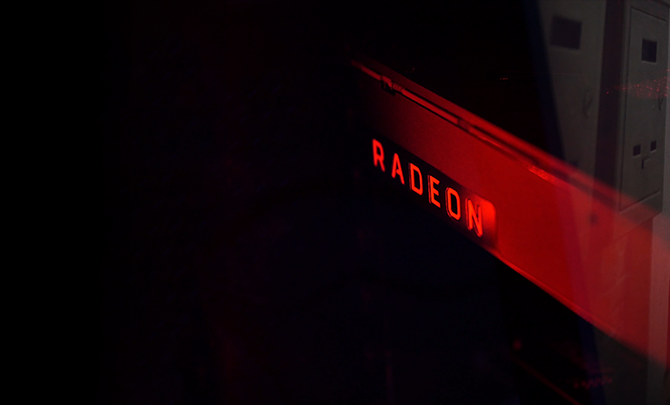
\includegraphics[width=\paperwidth,height=\paperheight]{gpu_background_black.png}
%% }
\pgfdeclareimage[width=\paperwidth]{mybackground}{gpu_background_black.png}
\setbeamertemplate{title page}{
  \begin{picture}(0,0)
    \put(-30,-163){%
      \pgfuseimage{mybackground}
    }
    \put(0,-150){%
      \begin{minipage}[b][45mm][t]{226mm}
        \usebeamerfont{title}{\inserttitle\par}
        \ifx\insertsubtitle\@empty%
        \else%
        {\vskip0.25em%
        \usebeamerfont{subtitle}\usebeamercolor[fg]{subtitle}\insertsubtitle\par}%
        \fi%
        \vskip1cm%              
        \usebeamerfont{author}{\insertauthor\par}
        \usebeamerfont{date}\url{malcolm.roberts@amd.com}\par
        \usebeamerfont{date}\insertdate
      \end{minipage}
    }
  \end{picture}
}

%------------------------------------------------------------------------
%------------------------------------------------------------------------



\def\thetitle{rocFFT}
\def\thesubtitle{An open-source GPU FFT Library for Exascale Systems}
\def\theauthor{Malcolm Roberts, Fei Zheng, and Bragadeesh Natarajan}
\def\theauthorinstitute{AMD}

\def\presdate{2020-02-14}

\hypersetup{
  pdftitle=\thetitle{} \thesubtitle{},
  pdfauthor=\theauthor{}
}

\title{\thetitle{}}
\subtitle{\thesubtitle{}}
\author{\theauthor{}}
\institute{\theauthorinstitute}
\date{\presdate}

\setbeamertemplate{frametitle}[default][center]
%\setbeamertemplate{footline}[frame number]
\setbeamertemplate{navigation symbols}{} 

\begin{document}

\setbeamertemplate{headline}{}
%\setbeamertemplate{footline}{}

{
  \setbeamercolor{background canvas}{bg=black}
  \setbeamercolor{normal text}{fg=white,bg=black}
  \setbeamercolor{frametitle}{fg=white}
  \setbeamercolor{title}{fg=white}
  \setbeamercolor{alerted text}{fg=white}
  \setbeamercolor{structure}{fg=white}
  \usebeamercolor[fg]{normal text}
  \begin{frame}
    \titlepage
  \end{frame}
}


\setbeamercolor{normal text}{fg=black,bg=white}
\usebeamercolor[fg]{normal text}

\newcolumntype{R}{>{\raggedleft\arraybackslash}X}
\setbeamertemplate{footline}{
   \leavevmode%
   \hbox{%
     \begin{beamercolorbox}[wd=\paperwidth,ht=1ex,dp=1.125ex]{author in head/foot}%
  \begin{tabularx}{\paperwidth}{lR}
    \hfill\insertframenumber/\inserttotalframenumber\hfill\phantom{.}%
    & %
    
\includegraphics[width=0.05\textwidth]{footerlogo}%
    \\%
  \end{tabularx}%
  \end{beamercolorbox}%
  }%
}

\begin{frame}
    \frametitle{Outline}

    \begin{itemize}
      
    \item ROCm: Radeon Open Compute Platform
    \item The \texttt{HIP} programming language
    \item \texttt{rocFFT}
      \begin{itemize}
        \item Design
        \item Features
        \item Usage
      \end{itemize}
    \item Sample applications
    \end{itemize}
      
\end{frame}

\begin{frame}
    \frametitle{ROCm: Radeon Open Compute}

    \begin{center}
      \url{https://rocm.github.io/}
    \end{center}

    \begin{columns}
      \begin{column}{0.48\textwidth}
        \begin{itemize}
        \item Open source drivers and libraries
          \begin{itemize}
          \item Community engagement encouraged!
          \end{itemize}
        \item HPC and machine learning applications
        \item Focus on multi-gpu computation
        \item Some libraries of interest to the HPC community:
          \begin{itemize}
          \item rocBLAS
          \item rocSPARSE: sparse BLAS
          \item rocALUTION: sparse solvers
          \item rocFFT
          \end{itemize}
        \item Written in the HIP programming language
        \end{itemize}
      \end{column}
      \begin{column}{0.48\textwidth}
        
\includegraphics[width=0.9\textwidth]{ROCm-300x300.png}
        % FIXME: add logo ROCm_Logo_128.png
      \end{column}
    \end{columns}
      

    
\end{frame}

\begin{frame}
  \frametitle{HIP: Heterogeneous-Computing Interface for Portability}

  \begin{center}
    HIP is a \texttt{C++} dialect for GPU programming.
  \end{center}
  
  \bigskip
  
  \begin{center}
    Sample differences between HIP, CUDA, and OpenCL:
    \medskip
    
    \begin{tabular}{llll}
      Term & HIP & CUDA & OpenCL \\ \hline
      Device kernel &
      \lstinline[]$__global__$ &
      \lstinline[]$__global__$ &
      \lstinline[]$__kernel$ \\
      Thread index &
      \lstinline[]$threadIdx.x$ &
      \lstinline[]$threadIdx.x$ &
      \lstinline[]$get_local_id(0)$ \\
      Kernel launch &
      \lstinline[]$hipLaunchKernelGGL$ &
      \lstinline[]$<<< >>>$ &
      \lstinline[]$clEnqueueNDRangeKernel$ \\
    \end{tabular}
  \end{center}

  \bigskip
  
  \begin{center}
  The hipify tool converts CUDA code to HIP code.

  \medskip
  
  OpenCL continues to be supported.
  \end{center}

  \bigskip

  Compiler is a branch of \texttt{clang}, and will be upstreamed.
  
\end{frame}


\begin{frame}
    \frametitle{rocFFT: An open-source GPU FFT Library for Exascale Systems}

    \begin{center}
       \url{github.com/ROCmSoftwarePlatform/rocFFT}
    \end{center}

    \bigskip
    
    \begin{itemize}
    \item Open source:
      \medskip
    \item Written in \texttt{C++} and \texttt{HIP}
      \medskip
    \item can also be compiled with \texttt{nvcc}
      \medskip
    \item \texttt{rocfft} interface provides flexibility
      \medskip
    \item Alternative \texttt{hipfft} interface: usage similar to \texttt{cufft}
    \end{itemize}
    
\end{frame}

\begin{frame}
    \frametitle{rocFFT: design}

    \texttt{rocfft.h} provides a \texttt{C} interface.

    Based on the input parameters, we create a tree structure:
    \begin{itemize}
    \item Input and output buffers, strides, etc are assigned recursively.
    \item Leaf nodes contain device kernels.
    \item A plan is executed by traversing the leaf nodes sequentially.
    \end{itemize}

    \medskip
    
    Most kernels are generated.
    
    \medskip
    
    Kernel types:
    \begin{itemize}
    \item Stockham
    \item Transpose
    \item Bluestein
    \item Real/complex stages.
    \end{itemize}

    The host code is stored in \texttt{librocfft.so}; device kernels are in
    \texttt{librocfft-device.so}.
    
\end{frame}

\begin{frame}
    \frametitle{rocFFT: features}

    \begin{itemize}
    \item 1D, 2D, and 3D, transforms.
      \medskip
    \item Batched transforms.
      \medskip
    \item Single and double precision.
      \medskip
    \item In-place and out-of-place transforms.
      \medskip
    \item Input and output strides.
      \medskip
    \item Complex data format: interleaved or planar (aka ``split'').
      \medskip
    \item Extensive testing on several Linux distributions.
    \end{itemize}

\end{frame}


\begin{frame}
    \frametitle{rocFFT: usage}

    \begin{center}
      The \texttt{rocfft} interface is defined in \texttt{rocfft.h}.
    \end{center}
    
    \begin{enumerate}
    \item \lstinline[]$rocfft_setup()$
    \item Optional: create a \lstinline[]$rocfft_plan_description$ for advanced stride and
      other format choices.
    \item Create a \lstinline[]$rocfft_plan$, possibly using the description above.
    \item Create a \lstinline[]$rocfft_execution_info$
      \begin{enumerate}
      \item Get the scratch memory requirements of the \lstinline[]$rocfft_plan$
      \item Allocate the work buffer and associate it to the \lstinline[]$rocfft_execution_info$
      \end{enumerate}
    \item Allocate the input and output buffers and set up the input data.
    \item Execute the plan with \lstinline[]$rocfft_execute$.
    \item Free the buffers, destroy the \texttt{rocFFT} structures, and
      \lstinline[]$rocfft_cleanup()$.
    \end{enumerate}
    

\end{frame}

\begin{frame}[fragile]
    \frametitle{rocFFT: rocfft interface example}

\begin{lstlisting}
// create the plan:      
rocfft_plan_create(&plan,    
                   rocfft_placement_inplace,
                   rocfft_transform_type_complex_forward,
                   rocfft_precision_double,
                   1,       // dimension
                   &length, // transform lengths (column-major)
                   1,       // batch size
                   NULL);   // optional description

// allocate the work memory and associate it to the execution info:                 
rocfft_execution_info_create(&planinfo);
rocfft_plan_get_work_buffer_size(gpu_plan, &wsize);
hipMalloc(&wbuffer, wsize);
rocfft_execution_info_set_work_buffer(planinfo, wbuffer, wsize);

// execute the plan:
rocfft_execute(gpu_plan, gpu_in, planinfo);
\end{lstlisting}
\end{frame}
    
\begin{frame}[fragile]
    \frametitle{rocFFT: hipfft interface example}

\begin{lstlisting}
// Create the plan:
hipfftPlan1d(&plan,      // plan handle
             Nx,         // transform lengths
             HIPFFT_Z2Z, // transform type (HIPFFT_C2C for float)
             1);         // number of transforms
// Can also call hipfftPlanMany (row-major)
             
// Work memory is automatically created and associated with the plan.

// Execute the plan:
hipfftExecZ2Z(plan, x, x, direction);
\end{lstlisting}

\end{frame}


%% \begin{frame}
%%   \frametitle{rocFFT benchmarks}

%%   \begin{center}
%%     Tests were performed on the Radeon Instinct MI60.
%%   \end{center}

  
%%   FIXME
  
%% \end{frame}

\begin{frame}
  \frametitle{Frontier CAAR Projects}

  Some CAAR (Center for Accelerated Application Readiness) applications which target
  Frontier and which use FFTs (\url{www.olcf.ornl.gov/caar/frontier-caar}):

  \bigskip

  \begin{itemize}
  \item {GESTS (GPUs for Extreme-Scale Turbulence Simulations)}

    High-resolution pseudospectral code: 35 trillion grid points.

    \medskip
    
  \item{NAMD (Nanoscale Molecular Dynamics)}

    Molecular simulator; can use rocFFT as the backend.

        \medskip
  \item{PIConGPU (Particle-in-cell on Graphics Processing Units)}

    Plasma simulator: PIC methods often use FFTs to resolve the underlying Maxwell
    equations.
  \end{itemize}
  
\end{frame}


\begin{frame}[fragile]
  \frametitle{Conclusion}

  \begin{center}
    rocFFT is:
  \end{center}
  \bigskip
  \begin{itemize}
  \item An open-source GPU FFT library from AMD
  \medskip
  \item Part of ROCm: the Radeon Open Compute Platform
  \medskip
  \item Uses the HIP programming language
  \medskip
  \item Will be used by a number of applications for exascale computing.
  \end{itemize}

  \bigskip
  \begin{center}
    Available at: \url{github.com/ROCmSoftwarePlatform/rocFFT}
  \end{center}
  
\end{frame}

\end{document}

%%  LocalWords:  ROCm Radeon rocFFT HPC gpu rocBLAS rocSPARSE BLAS rocALUTION CUDA OpenCL
%%  LocalWords:  llll threadIdx hipLaunchKernelGGL clEnqueueNDRangeKernel hipify FFT nvcc
%%  LocalWords:  upstreamed Exascale rocfft hipfft cufft Stockham Bluestein librocfft Nx
%%  LocalWords:  inplace planinfo wsize hipMalloc wbuffer hipfftPlan hipfftPlanMany CAAR
%%  LocalWords:  hipfftExecZ Center FFTs GESTS GPUs pseudospectral NAMD Nanoscale backend
%%  LocalWords:  PIConGPU exascale
